% Chapter Template

\chapter{Background} % Main chapter title

\label{Background} % Change X to a consecutive number; for referencing this chapter elsewhere, use \ref{ChapterX}

%----------------------------------------------------------------------------------------
%	ASR
%----------------------------------------------------------------------------------------

\section{Automatic Speech Recognition}

Automatic speech recognition models can be split into two broad categories of complexity. First of all, there is single-word classification to an isolated vocabulary where directed dialogue conversations are analyzed; its functionality can be seen in early speech recognition efforts such as IBM’s Shoebox. The other variant is continuous speech recognition, where natural language conversations (NLCs) are processed and transcripted to a vocabulary of around 20,000 to 100,000 words. Many technologies today utilize this system, including video subtitles, voice searching, and customer services at call centres. Directed dialogue classification models can be fairly simple to understand and produce through various feed-forward networks, but natural language networks require the use of recurrent neural networks.

%-----------------------------------
%	RNN
%-----------------------------------
\section{Recurrent Neural Networks for ASR}

Recurrent neural networks are a variant of deep learning neural networks that use time-sequential data without a fixed shape. These systems are inspired by the biological composition of neurons in the brain, as humans have learned long ago to adapt their innovations from nature. Each neuron, out of around 100 million, is interconnected to many other neurons and passes a signal via its axon to receiving axon terminals belonging to other neurons. Contrastingly, in an artificial neural network, a combination of weights and biases stacked in layers are constantly optimized through gradient descent to produce a matrix of probabilities that highlight the best possible output the network can generate at its current state (for the case of classification architectures). In each cell, a dot product of the input matrix and the cell’s weight matrix is done and summed with the cell’s bias matrix to create an output matrix of values, fed into all of the nodes in the next layer. At first, these matrices use senseless, randomly generated weights and biases that result in a completely random output. However, as the model calculates its loss from an evaluation of the net deviation of the predicted output from the ground truth, a gradient is formulated that adjusts each layer’s parameters closer to what would create an output with a lower loss. The higher loss an output receives, the greater magnitude of the gradient is passed to backpropagation and the more each node is changed, with the vice versa applying as well.
\newline\par
In a typical multi-layer deep learning neural network, the input and output shape of the model are fixed and have to be set. Since the length of the NLC audio input is indeterminate in this investigation, recurrent neural networks can be used to process continuous speech data that last an indeterminate length of time. RNNs accomplish this task by accepting an input for each time step into a recurrent cell and feeding the cell’s generated output to the succeeding cell through a hidden layer, doing so until the input data is completely used. This results in the coupled nature of a recurrent neural network that enables it to find relationships in continuous data, namely in stock market prediction, and influence future outputs. The framework of a standard RNN cell is laid out below (Figure 2.1).

\begin{figure}[th]
    \centering
    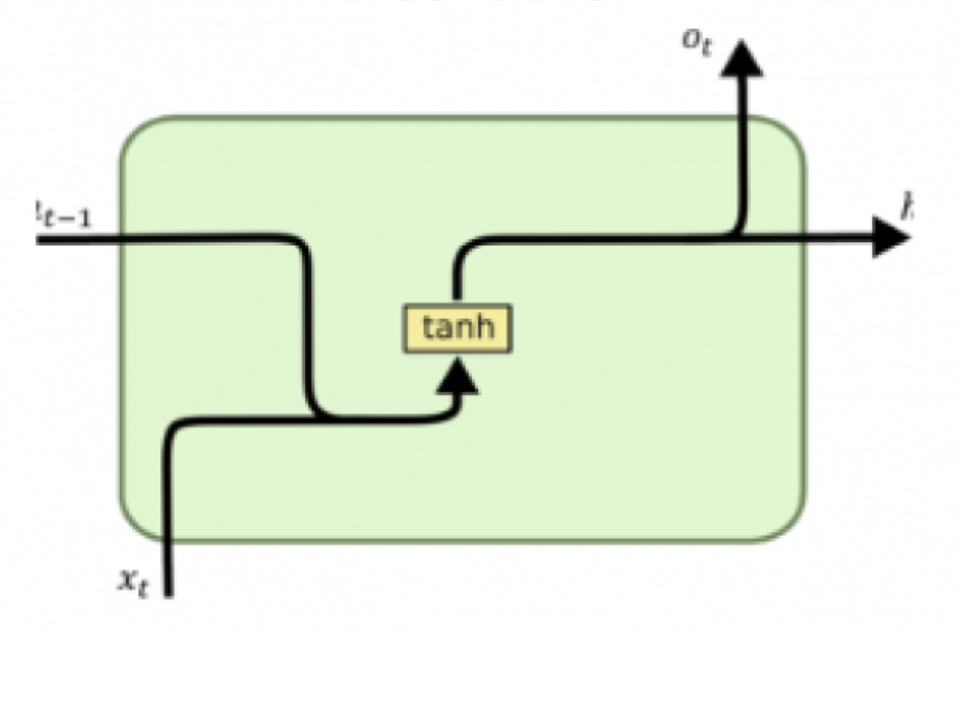
\includegraphics[width=0.5\textwidth]{Figures/rnnarch.png}
    \[ h_t = \tanh(W(
        \begin{pmatrix}
            h_{t-1} \\ x_t
        \end{pmatrix}
    )) \]
    \decoRule
    \caption[RNN Cell]{The internal composition of a hyperbolic tan RNN cell}
    \label{fig:RNNCell}
\end{figure}

The distribution of input data and output data can vary from network to network and is ultimately based on the shape of the input data and the desired shape of the output data. For example, a music generation RNN could take in a dataset of Vivaldi’s works as an input and output an infinite length of completely original Vivaldi-styled music: this model would be classified as a one-to-many RNN structure. The following table (Table 2.1) describes four main types of RNN structures that satisfy most machine learning purposes.

\begin{table}
    \centering
    \begin{tabular}{p{0.16\textwidth}p{0.23\textwidth}p{0.24\textwidth}p{0.15\textwidth}}
        \toprule
        \textbf{Architecture} & \textbf{Characteristics} & \textbf{Application} & \textbf{Diagram} \\
        \midrule

        One-to-One & Single input \newline Single output & Image classification & 
        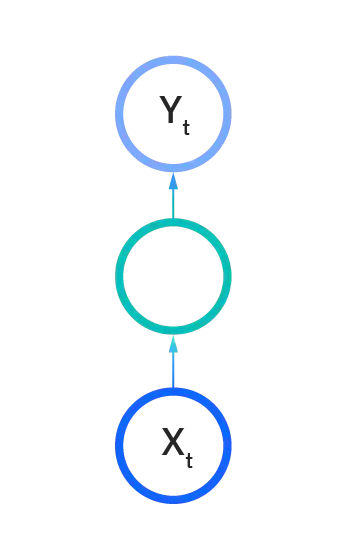
\includegraphics[width=0.08\textwidth]{Figures/onetoone.png} \\

        One-to-Many & Single input \newline Sequence of outputs & Image captioning & 
        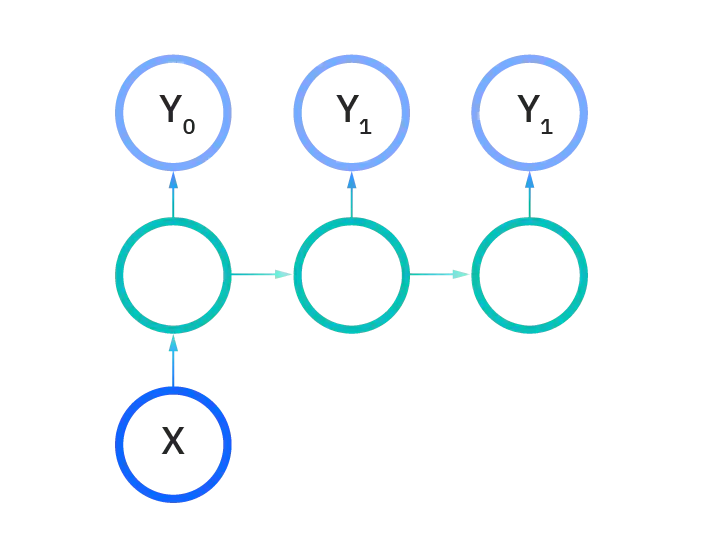
\includegraphics[width=0.16\textwidth]{Figures/onetomany.png} \\

        Many-to-One & Sequence of inputs \newline Single output & Sentiment analysis & 
        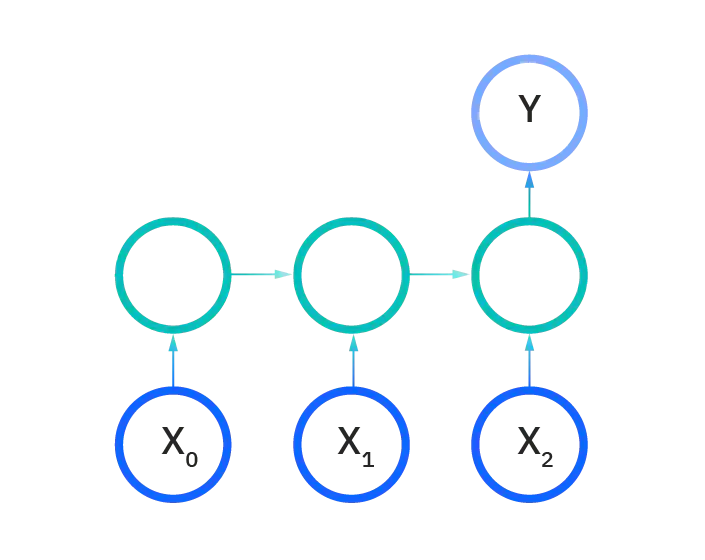
\includegraphics[width=0.16\textwidth]{Figures/manytoone.png} \\

        Many-to-Many & Sequence of inputs \newline Sequence of outputs & Language translation & 
        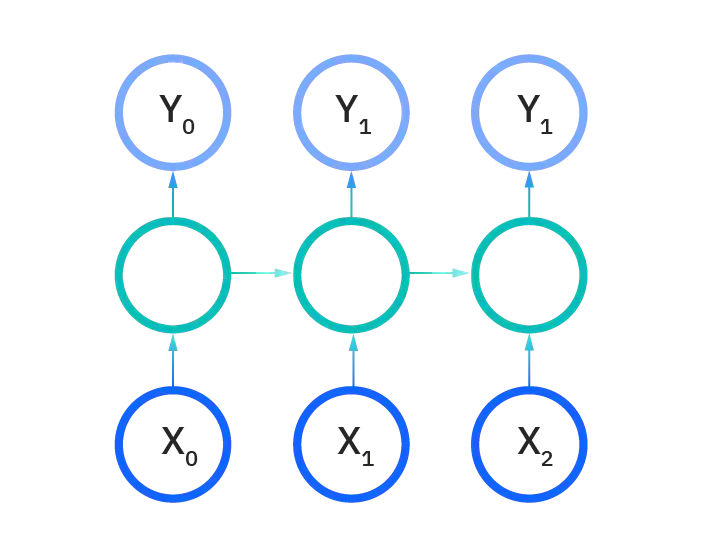
\includegraphics[width=0.16\textwidth]{Figures/manytomany.png} \\

        \bottomrule\\
    \end{tabular}
    \caption{Four types of recurrent neural network structures}
    \label{tab:RNNStructures}
\end{table}

Due to the continuous nature of NLC, multiple inputs as the audio data and its respective outputs as phonemes, letters, or words are present. Thus, a many-to-many structure will be used as the framework for this investigation’s experimentation.
\newline\par
However, conventional recurrent neural networks have two major problems that need to be considered: the vanishing and exploding gradient problem, and the long-term dependency on sound signals. The vanishing and exploding gradient problem appear during the backpropagation stage of the network, where a gradient propagates through each cell and updates the weights and biases of each node in order for the network to learn. The problem arises when the number of layers starts to increase and the gradients start to travel and multiplied through more and more layers; when a gradient with a slight deviation from y=x is returned to the first node during backpropagation, it begins to increase or decrease exponentially (dependent on its sign) as it progresses through each cell. Correspondingly, as it reaches near the end of backpropagation, the gradient is either too minuscule to the point where the end weight is scarcely updated at all, or too large where the weight cannot be optimized properly.
\newline\par
Going on, sound signals can take up a significant portion of input data, dependent on sample frequency, as a one-second audio clip of someone dictating a word can take up to 16,000 time steps of data. The extreme short-term memory of a simple hyperbolic tangent recurrent network cannot remember what sound signal was inputted into the cell some 5,000 iterations earlier, to the extent it is significant towards producing the output. This is detrimental towards the ultimate performance of the neural network, as a large segment of a model’s decision on a phoneme, character, or word depends on contextual data beforehand. For example, a model could have a hard time discriminating between the letter “k” and “q” with no context. However, the prerequisite knowledge that it was preceded by a “loo” will likely increase the probability that the following letter is “k”. These two setbacks of recurrent neural networks introduced a revolutionary recurrent cell concept introduced in 1997 and prominently used today, termed the Long Short-Term Memory cell.

%-----------------------------------
%	LSTM
%-----------------------------------
\section{Long Short-Term Memory}

Long Short-Term Memory cells counter the two problems above by incorporating an extra hidden memory state that propagates throughout recurrences of the network. The addition of a memory state that can remember important specifics from many recurrences beforehand and influence the current output. Contrary to the perception-based framework of traditional neural networks, an LSTM cell is much more convoluted and contains substantially more weights and biases in the form of specialized gates (Figure 2.2). The combination of these properties provides the fundamental framework that conceives the LSTM network’s ability to recognize context-sensitive information and is thus the reason why these networks are the standard for building reliable speech recognition systems. 

\begin{figure}[th]
    \centering
    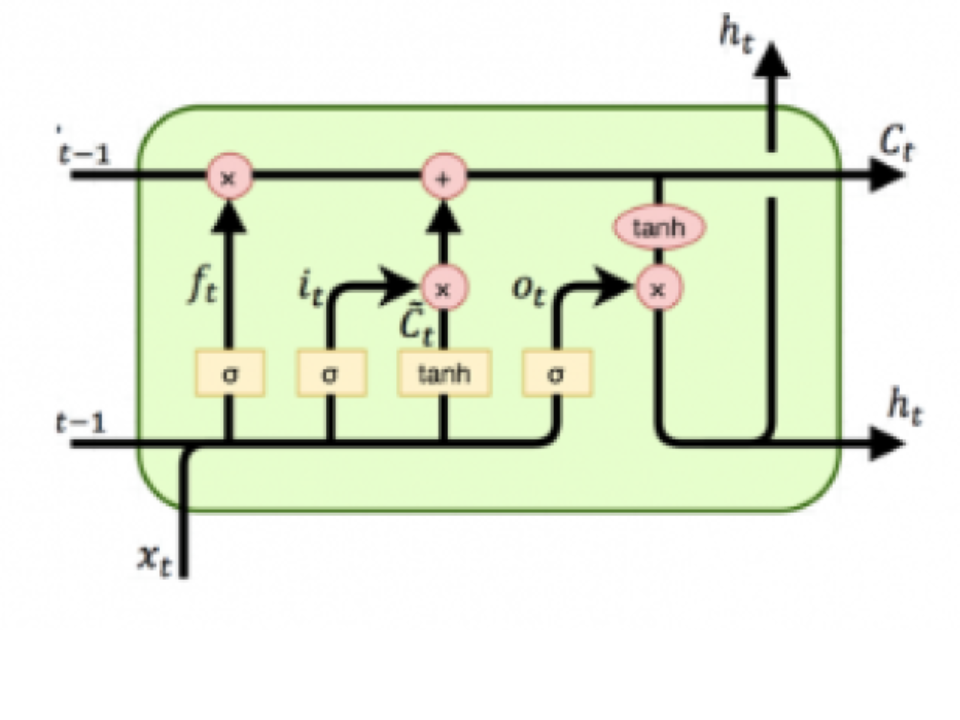
\includegraphics[width=0.5\textwidth]{Figures/lstmarch.png}
    \begin{displaymath}
    \begin{pmatrix}
        i_{gate} \\ f_{gate} \\ o_{gate} \\ g_{gate}
    \end{pmatrix}
    =
    \begin{pmatrix}
        \sigma \\ \sigma \\ \sigma \\ \tanh
    \end{pmatrix}
    W
    \begin{pmatrix}
        h_{t-1} \\ x_t
    \end{pmatrix} \\
    c_t = f \cdot c_{t-1} + i \cdot g \\
    h_t = o \cdot \tanh(c_t)
    \end{displaymath} \\
    \decoRule
    \caption[LSTM Cell]{The internal composition of an LSTM cell}
    \label{fig:LSTMCell}
\end{figure}

A simple speech recognition system is usually composed of two different components; a feature extraction layer and the neural network itself. The purpose of the feature extraction layer is to process the raw input data into a more usable and space-efficient form. In the case of ASR, input data is usually in the form of waveform data embedded in .mp3 or .wav files. This one-dimensional waveform data has several limitations due to having less useful features than a two-dimensional format of audio signals, such as spectrograms. Spectrograms are a visual representation of the amplitudinal spectrum of frequencies of an audio signal with respect to time. These isolated frequency amplitudes are also called the Discrete Fourier Transform (DFT) of an input and they can be extracted via the Fast Fourier Transform (FFT) algorithm, laid out below.
\newline\par
DFTs are frequently used in convolutional neural networks due to their property to be represented as an image and are the reliable standard in terms of extracting audio features from waveform data. In a DFT, the x-axis refers to time and the y-axis refers to the frequency that’s played at a certain point in time, with a lighter colour indicating that the amplitude is larger with regard to magnitude (Figure 2.3).

\begin{figure}[th]
    \centering
    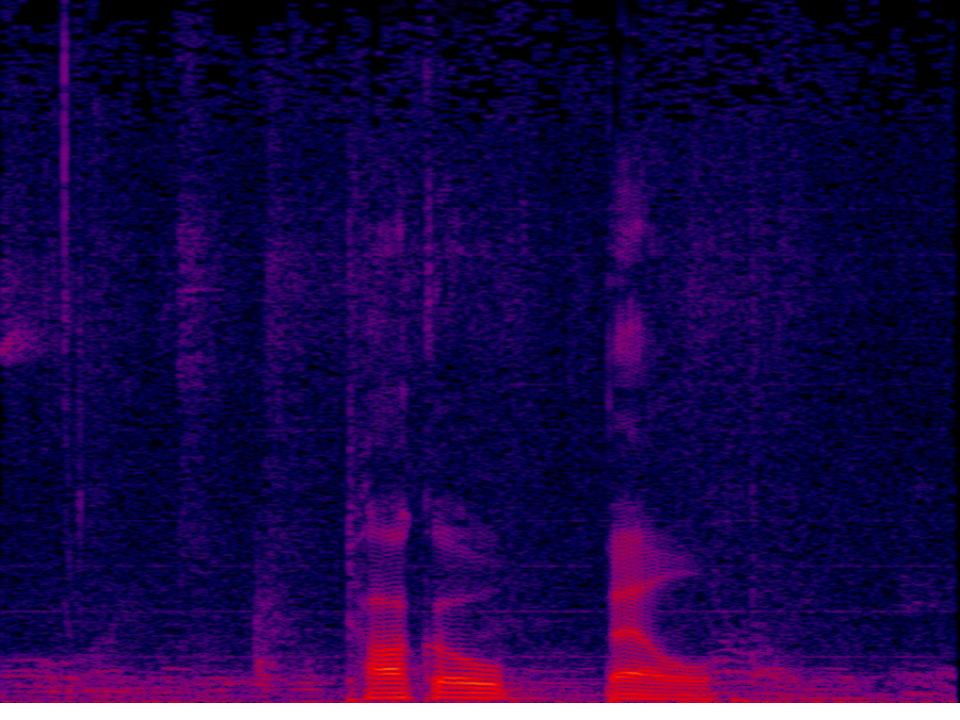
\includegraphics[width=0.5\textwidth]{Figures/tacobell.png}
    \decoRule
    \caption[Spectrogram]{A spectrogram of a person saying the phrase, "Taco Bell"}
    \label{fig:Spectrogram}
\end{figure}

%-----------------------------------
%	Feature Extraction Algorithms
%-----------------------------------
\section{Feature Extraction Algorithms}

However, spectrograms are not very well suited nor optimized for visualizing human speech. For instance, a human voice at a conversational level will normally not exceed a frequency of 500 Hz and fall below 60 Hz and it’s not necessary to include non-phonetically vital properties of speech signals in the input data. Therefore, Mel Frequency Cepstral Coefficients (MFCC) intended to artificially replicate the human hearing system with the assumption that the human ear is a reliable speech recognition system in itself. A precise logarithm function is used to retain the phonetically vital properties of speech signals and plot the result on the Mel scale (below).

\[mel(f) = 2595 x \log_10(1+ f/700)\]

MFCCs are created first by passing spectrogram data through a precise logarithm function, dubbed the Mel-filter bank, to retain the phonetically vital properties of speech signals while also reducing the number of unwanted frequencies in our input data. The result is plotted to a Mel spectrum and applied to the inverse discrete cosine transform, in which it is finally converted into a cepstrum, the inverse of a spectrum. The result is a set of 10-21 coefficients that ultimately present the main speech features of the original waveform data. MFCC data can also be taken as the derivative of and provide further feature data to feed into the neural network.
\newline\par
Other speech feature extraction functions that will be investigated are DWT, LPC, and PLP. They are each unique in their own manner but are also very closely related to each other with reference to the algorithms used to create them. Discrete Wavelet Transforms decompose a signal into a set of mutually orthogonal wavelet basis functions. It uses the Short-Time Fourier Transform, a variant of the FFT, which carries out a Fourier transform on a signal split into small windows of fixed duration instead of a specific time instance. Linear Predictive Coding generates coefficients that, similar to MFCCs, reflect the characteristics of a simplified vocal tract model, overall compressing the signal alongside the process. As the name suggests, the method is competent at predicting the future of a random process given past observations. Finally, Perceptual Linear Prediction claims to improve speaker-independent recognition performance and outperform LPCs in speech recognition. It first warps the spectrogram along the Bark frequency scale (Figure 2.4), convolves it with the power spectrum, and performs a cubic-root amplitude compression, ultimately creating the linear prediction model.

\begin{figure}[th]
    \centering
    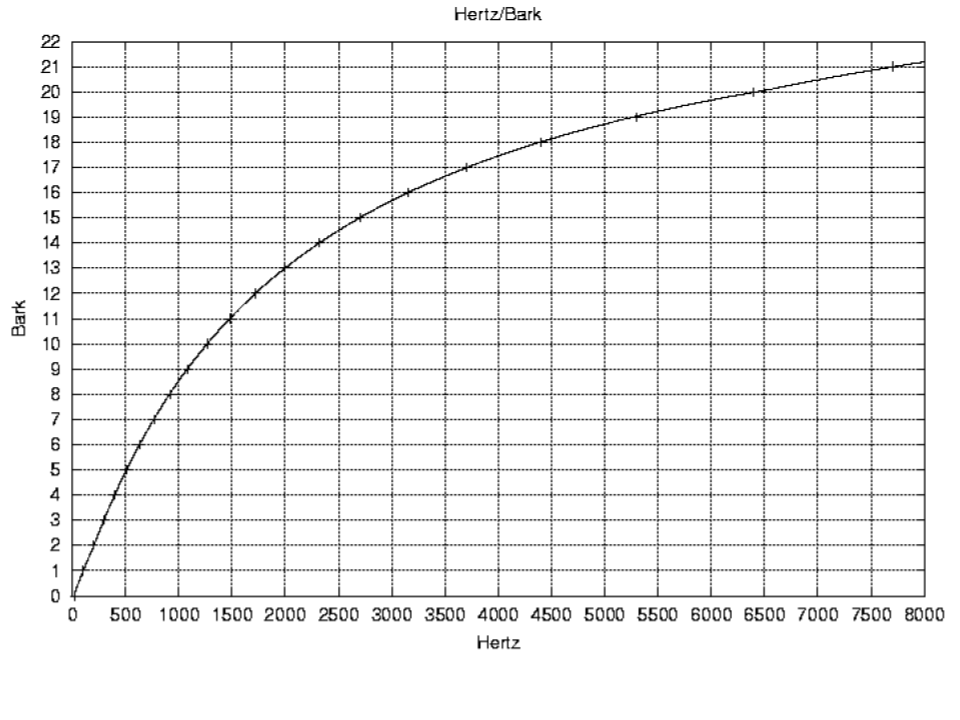
\includegraphics[width=0.5\textwidth]{Figures/barkscale.png}
    \decoRule
    \caption[Bark Scale]{The Bark scale, visualized on a graph comparing Bark value and frequency}
    \label{fig:BarkScale}
\end{figure}